\usubsection{Caso 3}

\usubsubsection{Solución Teórica}

\begin{align*}
  R&=5k\Omega&
  C&=470\mu F&
  L&=5mH
\end{align*}
En este caso $t_0=0$.
\begin{align*}
  s_1 &= \frac{-\frac{5k\Omega}{5mH}
  - \sqrt{\left(\frac{5k\Omega}{5mH}\right)^2-\frac{4}{5mH470\mu F}}}{2}
  &
  s_2 &= \frac{-\frac{5k\Omega}{5mH}
  + \sqrt{\left(\frac{5k\Omega}{5mH}\right)^2-\frac{4}{5mH470\mu F}}}{2}
\end{align*}

\usubsubsection{Simulación}

\begin{figure}[H]
  \lstinputlisting{modelica/RLCSerie3.mo}
  \caption{Código para el tercer caso.}
\end{figure}

\begin{figure}[H]
  \centering
  \label{gr:caso1:corrientes}
  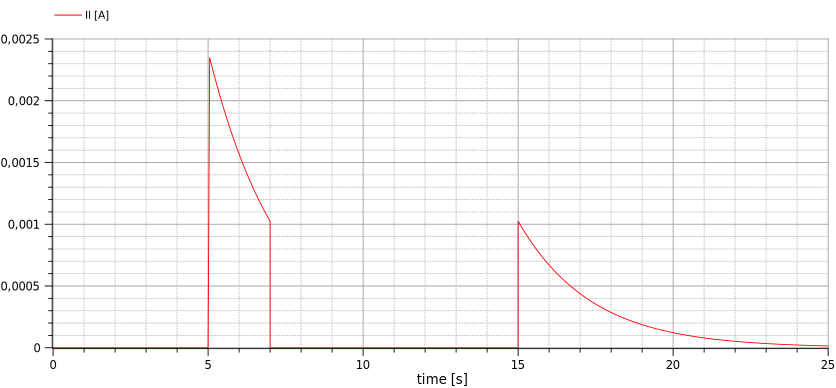
\includegraphics[width=\textwidth]{modelica/graficas/3-corrientes}
  \caption{Gráfica de Corrientes para el tercer caso.}
\end{figure}

\begin{figure}[H]
  \centering
  \label{gr:caso1:tensiones}
  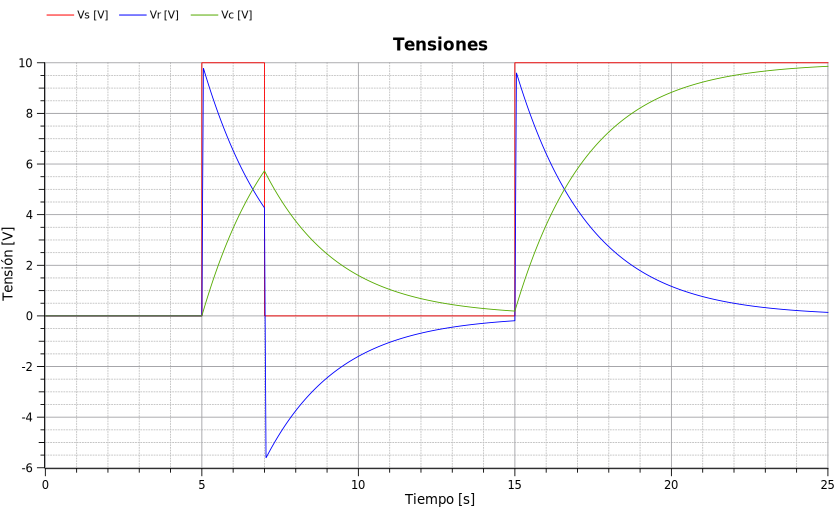
\includegraphics[width=\textwidth]{modelica/graficas/3-tensiones}
  \caption{Gráfica de Tensiones para el tercer caso.}
\end{figure}
